
% Default to the notebook output style

    


% Inherit from the specified cell style.




    
\documentclass[11pt]{article}

    
    
    \usepackage[T1]{fontenc}
    % Nicer default font (+ math font) than Computer Modern for most use cases
    \usepackage{mathpazo}

    % Basic figure setup, for now with no caption control since it's done
    % automatically by Pandoc (which extracts ![](path) syntax from Markdown).
    \usepackage{graphicx}
    % We will generate all images so they have a width \maxwidth. This means
    % that they will get their normal width if they fit onto the page, but
    % are scaled down if they would overflow the margins.
    \makeatletter
    \def\maxwidth{\ifdim\Gin@nat@width>\linewidth\linewidth
    \else\Gin@nat@width\fi}
    \makeatother
    \let\Oldincludegraphics\includegraphics
    % Set max figure width to be 80% of text width, for now hardcoded.
    \renewcommand{\includegraphics}[1]{\Oldincludegraphics[width=.8\maxwidth]{#1}}
    % Ensure that by default, figures have no caption (until we provide a
    % proper Figure object with a Caption API and a way to capture that
    % in the conversion process - todo).
    \usepackage{caption}
    \DeclareCaptionLabelFormat{nolabel}{}
    \captionsetup{labelformat=nolabel}

    \usepackage{adjustbox} % Used to constrain images to a maximum size 
    \usepackage{xcolor} % Allow colors to be defined
    \usepackage{enumerate} % Needed for markdown enumerations to work
    \usepackage{geometry} % Used to adjust the document margins
    \usepackage{amsmath} % Equations
    \usepackage{amssymb} % Equations
    \usepackage{textcomp} % defines textquotesingle
    % Hack from http://tex.stackexchange.com/a/47451/13684:
    \AtBeginDocument{%
        \def\PYZsq{\textquotesingle}% Upright quotes in Pygmentized code
    }
    \usepackage{upquote} % Upright quotes for verbatim code
    \usepackage{eurosym} % defines \euro
    \usepackage[mathletters]{ucs} % Extended unicode (utf-8) support
    \usepackage[utf8x]{inputenc} % Allow utf-8 characters in the tex document
    \usepackage{fancyvrb} % verbatim replacement that allows latex
    \usepackage{grffile} % extends the file name processing of package graphics 
                         % to support a larger range 
    % The hyperref package gives us a pdf with properly built
    % internal navigation ('pdf bookmarks' for the table of contents,
    % internal cross-reference links, web links for URLs, etc.)
    \usepackage{hyperref}
    \usepackage{longtable} % longtable support required by pandoc >1.10
    \usepackage{booktabs}  % table support for pandoc > 1.12.2
    \usepackage[inline]{enumitem} % IRkernel/repr support (it uses the enumerate* environment)
    \usepackage[normalem]{ulem} % ulem is needed to support strikethroughs (\sout)
                                % normalem makes italics be italics, not underlines
    

    
    
    % Colors for the hyperref package
    \definecolor{urlcolor}{rgb}{0,.145,.698}
    \definecolor{linkcolor}{rgb}{.71,0.21,0.01}
    \definecolor{citecolor}{rgb}{.12,.54,.11}

    % ANSI colors
    \definecolor{ansi-black}{HTML}{3E424D}
    \definecolor{ansi-black-intense}{HTML}{282C36}
    \definecolor{ansi-red}{HTML}{E75C58}
    \definecolor{ansi-red-intense}{HTML}{B22B31}
    \definecolor{ansi-green}{HTML}{00A250}
    \definecolor{ansi-green-intense}{HTML}{007427}
    \definecolor{ansi-yellow}{HTML}{DDB62B}
    \definecolor{ansi-yellow-intense}{HTML}{B27D12}
    \definecolor{ansi-blue}{HTML}{208FFB}
    \definecolor{ansi-blue-intense}{HTML}{0065CA}
    \definecolor{ansi-magenta}{HTML}{D160C4}
    \definecolor{ansi-magenta-intense}{HTML}{A03196}
    \definecolor{ansi-cyan}{HTML}{60C6C8}
    \definecolor{ansi-cyan-intense}{HTML}{258F8F}
    \definecolor{ansi-white}{HTML}{C5C1B4}
    \definecolor{ansi-white-intense}{HTML}{A1A6B2}

    % commands and environments needed by pandoc snippets
    % extracted from the output of `pandoc -s`
    \providecommand{\tightlist}{%
      \setlength{\itemsep}{0pt}\setlength{\parskip}{0pt}}
    \DefineVerbatimEnvironment{Highlighting}{Verbatim}{commandchars=\\\{\}}
    % Add ',fontsize=\small' for more characters per line
    \newenvironment{Shaded}{}{}
    \newcommand{\KeywordTok}[1]{\textcolor[rgb]{0.00,0.44,0.13}{\textbf{{#1}}}}
    \newcommand{\DataTypeTok}[1]{\textcolor[rgb]{0.56,0.13,0.00}{{#1}}}
    \newcommand{\DecValTok}[1]{\textcolor[rgb]{0.25,0.63,0.44}{{#1}}}
    \newcommand{\BaseNTok}[1]{\textcolor[rgb]{0.25,0.63,0.44}{{#1}}}
    \newcommand{\FloatTok}[1]{\textcolor[rgb]{0.25,0.63,0.44}{{#1}}}
    \newcommand{\CharTok}[1]{\textcolor[rgb]{0.25,0.44,0.63}{{#1}}}
    \newcommand{\StringTok}[1]{\textcolor[rgb]{0.25,0.44,0.63}{{#1}}}
    \newcommand{\CommentTok}[1]{\textcolor[rgb]{0.38,0.63,0.69}{\textit{{#1}}}}
    \newcommand{\OtherTok}[1]{\textcolor[rgb]{0.00,0.44,0.13}{{#1}}}
    \newcommand{\AlertTok}[1]{\textcolor[rgb]{1.00,0.00,0.00}{\textbf{{#1}}}}
    \newcommand{\FunctionTok}[1]{\textcolor[rgb]{0.02,0.16,0.49}{{#1}}}
    \newcommand{\RegionMarkerTok}[1]{{#1}}
    \newcommand{\ErrorTok}[1]{\textcolor[rgb]{1.00,0.00,0.00}{\textbf{{#1}}}}
    \newcommand{\NormalTok}[1]{{#1}}
    
    % Additional commands for more recent versions of Pandoc
    \newcommand{\ConstantTok}[1]{\textcolor[rgb]{0.53,0.00,0.00}{{#1}}}
    \newcommand{\SpecialCharTok}[1]{\textcolor[rgb]{0.25,0.44,0.63}{{#1}}}
    \newcommand{\VerbatimStringTok}[1]{\textcolor[rgb]{0.25,0.44,0.63}{{#1}}}
    \newcommand{\SpecialStringTok}[1]{\textcolor[rgb]{0.73,0.40,0.53}{{#1}}}
    \newcommand{\ImportTok}[1]{{#1}}
    \newcommand{\DocumentationTok}[1]{\textcolor[rgb]{0.73,0.13,0.13}{\textit{{#1}}}}
    \newcommand{\AnnotationTok}[1]{\textcolor[rgb]{0.38,0.63,0.69}{\textbf{\textit{{#1}}}}}
    \newcommand{\CommentVarTok}[1]{\textcolor[rgb]{0.38,0.63,0.69}{\textbf{\textit{{#1}}}}}
    \newcommand{\VariableTok}[1]{\textcolor[rgb]{0.10,0.09,0.49}{{#1}}}
    \newcommand{\ControlFlowTok}[1]{\textcolor[rgb]{0.00,0.44,0.13}{\textbf{{#1}}}}
    \newcommand{\OperatorTok}[1]{\textcolor[rgb]{0.40,0.40,0.40}{{#1}}}
    \newcommand{\BuiltInTok}[1]{{#1}}
    \newcommand{\ExtensionTok}[1]{{#1}}
    \newcommand{\PreprocessorTok}[1]{\textcolor[rgb]{0.74,0.48,0.00}{{#1}}}
    \newcommand{\AttributeTok}[1]{\textcolor[rgb]{0.49,0.56,0.16}{{#1}}}
    \newcommand{\InformationTok}[1]{\textcolor[rgb]{0.38,0.63,0.69}{\textbf{\textit{{#1}}}}}
    \newcommand{\WarningTok}[1]{\textcolor[rgb]{0.38,0.63,0.69}{\textbf{\textit{{#1}}}}}
    
    
    % Define a nice break command that doesn't care if a line doesn't already
    % exist.
    \def\br{\hspace*{\fill} \\* }
    % Math Jax compatability definitions
    \def\gt{>}
    \def\lt{<}
    % Document parameters
    \title{balancing\_data}
    
    
    

    % Pygments definitions
    
\makeatletter
\def\PY@reset{\let\PY@it=\relax \let\PY@bf=\relax%
    \let\PY@ul=\relax \let\PY@tc=\relax%
    \let\PY@bc=\relax \let\PY@ff=\relax}
\def\PY@tok#1{\csname PY@tok@#1\endcsname}
\def\PY@toks#1+{\ifx\relax#1\empty\else%
    \PY@tok{#1}\expandafter\PY@toks\fi}
\def\PY@do#1{\PY@bc{\PY@tc{\PY@ul{%
    \PY@it{\PY@bf{\PY@ff{#1}}}}}}}
\def\PY#1#2{\PY@reset\PY@toks#1+\relax+\PY@do{#2}}

\expandafter\def\csname PY@tok@w\endcsname{\def\PY@tc##1{\textcolor[rgb]{0.73,0.73,0.73}{##1}}}
\expandafter\def\csname PY@tok@c\endcsname{\let\PY@it=\textit\def\PY@tc##1{\textcolor[rgb]{0.25,0.50,0.50}{##1}}}
\expandafter\def\csname PY@tok@cp\endcsname{\def\PY@tc##1{\textcolor[rgb]{0.74,0.48,0.00}{##1}}}
\expandafter\def\csname PY@tok@k\endcsname{\let\PY@bf=\textbf\def\PY@tc##1{\textcolor[rgb]{0.00,0.50,0.00}{##1}}}
\expandafter\def\csname PY@tok@kp\endcsname{\def\PY@tc##1{\textcolor[rgb]{0.00,0.50,0.00}{##1}}}
\expandafter\def\csname PY@tok@kt\endcsname{\def\PY@tc##1{\textcolor[rgb]{0.69,0.00,0.25}{##1}}}
\expandafter\def\csname PY@tok@o\endcsname{\def\PY@tc##1{\textcolor[rgb]{0.40,0.40,0.40}{##1}}}
\expandafter\def\csname PY@tok@ow\endcsname{\let\PY@bf=\textbf\def\PY@tc##1{\textcolor[rgb]{0.67,0.13,1.00}{##1}}}
\expandafter\def\csname PY@tok@nb\endcsname{\def\PY@tc##1{\textcolor[rgb]{0.00,0.50,0.00}{##1}}}
\expandafter\def\csname PY@tok@nf\endcsname{\def\PY@tc##1{\textcolor[rgb]{0.00,0.00,1.00}{##1}}}
\expandafter\def\csname PY@tok@nc\endcsname{\let\PY@bf=\textbf\def\PY@tc##1{\textcolor[rgb]{0.00,0.00,1.00}{##1}}}
\expandafter\def\csname PY@tok@nn\endcsname{\let\PY@bf=\textbf\def\PY@tc##1{\textcolor[rgb]{0.00,0.00,1.00}{##1}}}
\expandafter\def\csname PY@tok@ne\endcsname{\let\PY@bf=\textbf\def\PY@tc##1{\textcolor[rgb]{0.82,0.25,0.23}{##1}}}
\expandafter\def\csname PY@tok@nv\endcsname{\def\PY@tc##1{\textcolor[rgb]{0.10,0.09,0.49}{##1}}}
\expandafter\def\csname PY@tok@no\endcsname{\def\PY@tc##1{\textcolor[rgb]{0.53,0.00,0.00}{##1}}}
\expandafter\def\csname PY@tok@nl\endcsname{\def\PY@tc##1{\textcolor[rgb]{0.63,0.63,0.00}{##1}}}
\expandafter\def\csname PY@tok@ni\endcsname{\let\PY@bf=\textbf\def\PY@tc##1{\textcolor[rgb]{0.60,0.60,0.60}{##1}}}
\expandafter\def\csname PY@tok@na\endcsname{\def\PY@tc##1{\textcolor[rgb]{0.49,0.56,0.16}{##1}}}
\expandafter\def\csname PY@tok@nt\endcsname{\let\PY@bf=\textbf\def\PY@tc##1{\textcolor[rgb]{0.00,0.50,0.00}{##1}}}
\expandafter\def\csname PY@tok@nd\endcsname{\def\PY@tc##1{\textcolor[rgb]{0.67,0.13,1.00}{##1}}}
\expandafter\def\csname PY@tok@s\endcsname{\def\PY@tc##1{\textcolor[rgb]{0.73,0.13,0.13}{##1}}}
\expandafter\def\csname PY@tok@sd\endcsname{\let\PY@it=\textit\def\PY@tc##1{\textcolor[rgb]{0.73,0.13,0.13}{##1}}}
\expandafter\def\csname PY@tok@si\endcsname{\let\PY@bf=\textbf\def\PY@tc##1{\textcolor[rgb]{0.73,0.40,0.53}{##1}}}
\expandafter\def\csname PY@tok@se\endcsname{\let\PY@bf=\textbf\def\PY@tc##1{\textcolor[rgb]{0.73,0.40,0.13}{##1}}}
\expandafter\def\csname PY@tok@sr\endcsname{\def\PY@tc##1{\textcolor[rgb]{0.73,0.40,0.53}{##1}}}
\expandafter\def\csname PY@tok@ss\endcsname{\def\PY@tc##1{\textcolor[rgb]{0.10,0.09,0.49}{##1}}}
\expandafter\def\csname PY@tok@sx\endcsname{\def\PY@tc##1{\textcolor[rgb]{0.00,0.50,0.00}{##1}}}
\expandafter\def\csname PY@tok@m\endcsname{\def\PY@tc##1{\textcolor[rgb]{0.40,0.40,0.40}{##1}}}
\expandafter\def\csname PY@tok@gh\endcsname{\let\PY@bf=\textbf\def\PY@tc##1{\textcolor[rgb]{0.00,0.00,0.50}{##1}}}
\expandafter\def\csname PY@tok@gu\endcsname{\let\PY@bf=\textbf\def\PY@tc##1{\textcolor[rgb]{0.50,0.00,0.50}{##1}}}
\expandafter\def\csname PY@tok@gd\endcsname{\def\PY@tc##1{\textcolor[rgb]{0.63,0.00,0.00}{##1}}}
\expandafter\def\csname PY@tok@gi\endcsname{\def\PY@tc##1{\textcolor[rgb]{0.00,0.63,0.00}{##1}}}
\expandafter\def\csname PY@tok@gr\endcsname{\def\PY@tc##1{\textcolor[rgb]{1.00,0.00,0.00}{##1}}}
\expandafter\def\csname PY@tok@ge\endcsname{\let\PY@it=\textit}
\expandafter\def\csname PY@tok@gs\endcsname{\let\PY@bf=\textbf}
\expandafter\def\csname PY@tok@gp\endcsname{\let\PY@bf=\textbf\def\PY@tc##1{\textcolor[rgb]{0.00,0.00,0.50}{##1}}}
\expandafter\def\csname PY@tok@go\endcsname{\def\PY@tc##1{\textcolor[rgb]{0.53,0.53,0.53}{##1}}}
\expandafter\def\csname PY@tok@gt\endcsname{\def\PY@tc##1{\textcolor[rgb]{0.00,0.27,0.87}{##1}}}
\expandafter\def\csname PY@tok@err\endcsname{\def\PY@bc##1{\setlength{\fboxsep}{0pt}\fcolorbox[rgb]{1.00,0.00,0.00}{1,1,1}{\strut ##1}}}
\expandafter\def\csname PY@tok@kc\endcsname{\let\PY@bf=\textbf\def\PY@tc##1{\textcolor[rgb]{0.00,0.50,0.00}{##1}}}
\expandafter\def\csname PY@tok@kd\endcsname{\let\PY@bf=\textbf\def\PY@tc##1{\textcolor[rgb]{0.00,0.50,0.00}{##1}}}
\expandafter\def\csname PY@tok@kn\endcsname{\let\PY@bf=\textbf\def\PY@tc##1{\textcolor[rgb]{0.00,0.50,0.00}{##1}}}
\expandafter\def\csname PY@tok@kr\endcsname{\let\PY@bf=\textbf\def\PY@tc##1{\textcolor[rgb]{0.00,0.50,0.00}{##1}}}
\expandafter\def\csname PY@tok@bp\endcsname{\def\PY@tc##1{\textcolor[rgb]{0.00,0.50,0.00}{##1}}}
\expandafter\def\csname PY@tok@fm\endcsname{\def\PY@tc##1{\textcolor[rgb]{0.00,0.00,1.00}{##1}}}
\expandafter\def\csname PY@tok@vc\endcsname{\def\PY@tc##1{\textcolor[rgb]{0.10,0.09,0.49}{##1}}}
\expandafter\def\csname PY@tok@vg\endcsname{\def\PY@tc##1{\textcolor[rgb]{0.10,0.09,0.49}{##1}}}
\expandafter\def\csname PY@tok@vi\endcsname{\def\PY@tc##1{\textcolor[rgb]{0.10,0.09,0.49}{##1}}}
\expandafter\def\csname PY@tok@vm\endcsname{\def\PY@tc##1{\textcolor[rgb]{0.10,0.09,0.49}{##1}}}
\expandafter\def\csname PY@tok@sa\endcsname{\def\PY@tc##1{\textcolor[rgb]{0.73,0.13,0.13}{##1}}}
\expandafter\def\csname PY@tok@sb\endcsname{\def\PY@tc##1{\textcolor[rgb]{0.73,0.13,0.13}{##1}}}
\expandafter\def\csname PY@tok@sc\endcsname{\def\PY@tc##1{\textcolor[rgb]{0.73,0.13,0.13}{##1}}}
\expandafter\def\csname PY@tok@dl\endcsname{\def\PY@tc##1{\textcolor[rgb]{0.73,0.13,0.13}{##1}}}
\expandafter\def\csname PY@tok@s2\endcsname{\def\PY@tc##1{\textcolor[rgb]{0.73,0.13,0.13}{##1}}}
\expandafter\def\csname PY@tok@sh\endcsname{\def\PY@tc##1{\textcolor[rgb]{0.73,0.13,0.13}{##1}}}
\expandafter\def\csname PY@tok@s1\endcsname{\def\PY@tc##1{\textcolor[rgb]{0.73,0.13,0.13}{##1}}}
\expandafter\def\csname PY@tok@mb\endcsname{\def\PY@tc##1{\textcolor[rgb]{0.40,0.40,0.40}{##1}}}
\expandafter\def\csname PY@tok@mf\endcsname{\def\PY@tc##1{\textcolor[rgb]{0.40,0.40,0.40}{##1}}}
\expandafter\def\csname PY@tok@mh\endcsname{\def\PY@tc##1{\textcolor[rgb]{0.40,0.40,0.40}{##1}}}
\expandafter\def\csname PY@tok@mi\endcsname{\def\PY@tc##1{\textcolor[rgb]{0.40,0.40,0.40}{##1}}}
\expandafter\def\csname PY@tok@il\endcsname{\def\PY@tc##1{\textcolor[rgb]{0.40,0.40,0.40}{##1}}}
\expandafter\def\csname PY@tok@mo\endcsname{\def\PY@tc##1{\textcolor[rgb]{0.40,0.40,0.40}{##1}}}
\expandafter\def\csname PY@tok@ch\endcsname{\let\PY@it=\textit\def\PY@tc##1{\textcolor[rgb]{0.25,0.50,0.50}{##1}}}
\expandafter\def\csname PY@tok@cm\endcsname{\let\PY@it=\textit\def\PY@tc##1{\textcolor[rgb]{0.25,0.50,0.50}{##1}}}
\expandafter\def\csname PY@tok@cpf\endcsname{\let\PY@it=\textit\def\PY@tc##1{\textcolor[rgb]{0.25,0.50,0.50}{##1}}}
\expandafter\def\csname PY@tok@c1\endcsname{\let\PY@it=\textit\def\PY@tc##1{\textcolor[rgb]{0.25,0.50,0.50}{##1}}}
\expandafter\def\csname PY@tok@cs\endcsname{\let\PY@it=\textit\def\PY@tc##1{\textcolor[rgb]{0.25,0.50,0.50}{##1}}}

\def\PYZbs{\char`\\}
\def\PYZus{\char`\_}
\def\PYZob{\char`\{}
\def\PYZcb{\char`\}}
\def\PYZca{\char`\^}
\def\PYZam{\char`\&}
\def\PYZlt{\char`\<}
\def\PYZgt{\char`\>}
\def\PYZsh{\char`\#}
\def\PYZpc{\char`\%}
\def\PYZdl{\char`\$}
\def\PYZhy{\char`\-}
\def\PYZsq{\char`\'}
\def\PYZdq{\char`\"}
\def\PYZti{\char`\~}
% for compatibility with earlier versions
\def\PYZat{@}
\def\PYZlb{[}
\def\PYZrb{]}
\makeatother


    % Exact colors from NB
    \definecolor{incolor}{rgb}{0.0, 0.0, 0.5}
    \definecolor{outcolor}{rgb}{0.545, 0.0, 0.0}



    
    % Prevent overflowing lines due to hard-to-break entities
    \sloppy 
    % Setup hyperref package
    \hypersetup{
      breaklinks=true,  % so long urls are correctly broken across lines
      colorlinks=true,
      urlcolor=urlcolor,
      linkcolor=linkcolor,
      citecolor=citecolor,
      }
    % Slightly bigger margins than the latex defaults
    
    \geometry{verbose,tmargin=1in,bmargin=1in,lmargin=1in,rmargin=1in}
    
    

    \begin{document}
    
    
    \maketitle
    
    

    
    \begin{Verbatim}[commandchars=\\\{\}]
{\color{incolor}In [{\color{incolor}149}]:} \PY{o}{\PYZpc{}}\PY{k}{matplotlib} inline
          
          \PY{k+kn}{import} \PY{n+nn}{matplotlib}
          \PY{k+kn}{import} \PY{n+nn}{numpy} \PY{k}{as} \PY{n+nn}{np}
          \PY{k+kn}{import} \PY{n+nn}{pandas} \PY{k}{as} \PY{n+nn}{pd}
          \PY{k+kn}{from} \PY{n+nn}{sklearn}\PY{n+nn}{.}\PY{n+nn}{linear\PYZus{}model} \PY{k}{import} \PY{n}{LogisticRegression}
          \PY{k+kn}{from} \PY{n+nn}{sklearn}\PY{n+nn}{.}\PY{n+nn}{model\PYZus{}selection} \PY{k}{import} \PY{n}{train\PYZus{}test\PYZus{}split}
          \PY{k+kn}{from} \PY{n+nn}{sklearn}\PY{n+nn}{.}\PY{n+nn}{metrics} \PY{k}{import} \PY{n}{confusion\PYZus{}matrix}\PY{p}{,} \PY{n}{precision\PYZus{}recall\PYZus{}fscore\PYZus{}support}
          \PY{k+kn}{import} \PY{n+nn}{matplotlib}\PY{n+nn}{.}\PY{n+nn}{pyplot} \PY{k}{as} \PY{n+nn}{plt}
\end{Verbatim}


    \section{Handling Imbalanced Data}\label{handling-imbalanced-data}

\subsection{Introduction}\label{introduction}

In machine learning you typically want to build a model that does what
it is suppose to do.

If you have an image classifier, you want your model to correctly
classify images.

\begin{figure}
\centering
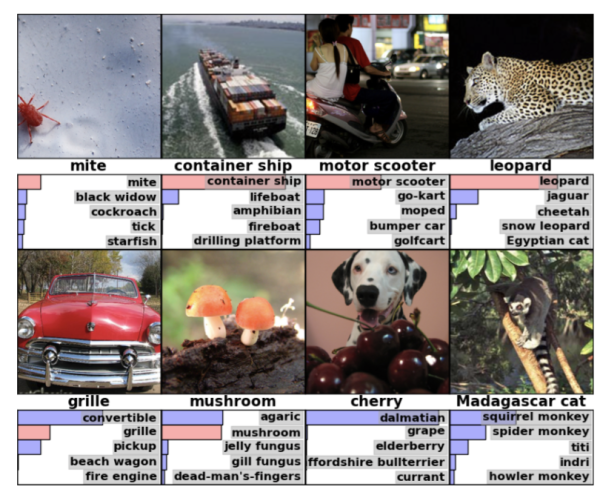
\includegraphics{../data/img/imagenet_example.png}
\caption{"https://www.google.ca/url?sa=i\&rct=j\&q=\&esrc=s\&source=images\&cd=\&cad=rja\&uact=8\&ved=2ahUKEwjToc6I8pDdAhVNCDQIHayCA9wQjRx6BAgBEAU\&url=https\%3A\%2F\%2Fblog.acolyer.org\%2F2016\%2F04\%2F20\%2Fimagenet-classification-with-deep-convolutional-neural-networks\%2F\&psig=AOvVaw3\_8QOTYYyy1ixeoaof-d\_z\&ust=1535584557428370"}
\end{figure}

So how do you determine how well your model is at doing its job?

With classification, for example, people generally take the proportion
of correctly classified images as the model's accuracy score.

\[Accuracy = \frac{\#\ of\ correctly\ classfied\ images}{\#\ of\ total\ classified\ images}\]

A high accuracy score usually equates to a good model.

\begin{figure}
\centering
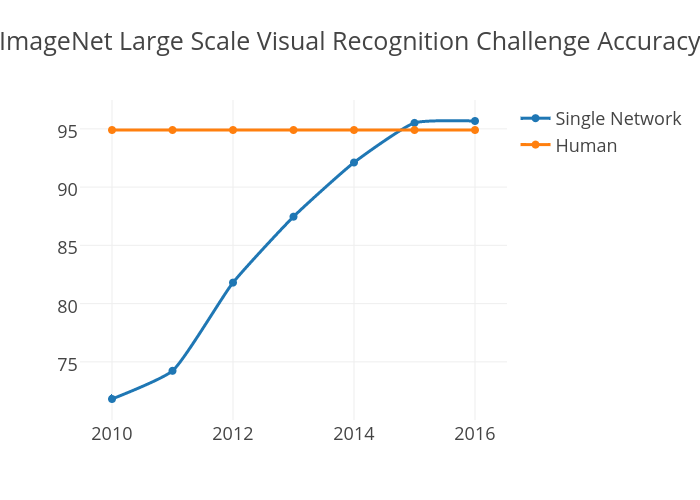
\includegraphics{../data/img/imagenet_scores.png}
\caption{"https://plot.ly/\textasciitilde{}botevmg/5/imagenet-large-scale-visual-recognition-challenge-accuracy.png"}
\end{figure}

\textbf{BUT... this is not always true...}

    \subsection{Welcome to healthcare}\label{welcome-to-healthcare}

Let's say you develop a binary classification model that aims to
determine a person's HIV status.

If this model is tested on every person in Canada and yields an overall
accuracy score of 99.7\%, would you consider the model worthy of
replacing traditional ways of testing for HIV?

\subsubsection{\texorpdfstring{\textbf{NOPE}}{NOPE}}\label{nope}

\paragraph{\texorpdfstring{\textbf{Sometimes the incorrect predictions
are more important than the correct
predictions}}{Sometimes the incorrect predictions are more important than the correct predictions}}\label{sometimes-the-incorrect-predictions-are-more-important-than-the-correct-predictions}

The prevelence of HIV/AIDS in Canada is 212 people per 100,000 (0.212\%)
\href{https://en.wikipedia.org/wiki/HIV/AIDS_in_Canada}{1}. This means
that 99.788\% of Canada's population is HIV negative.

If your model \textbf{predicts every person in Canada to be HIV
negative}, it would automatically result in an \textbf{accuracy score of
99.788\%}.

\[Accuracy = \frac{\#\ of\ correctly\ classfied\ images}{\#\ of\ total\ classified\ images}\]

\[Accuracy = \frac{100,000-212}{100,000}\]

\[Accuracy = 0.99788=99.788\%\]

The score seems good, but if we are more interested in correctly
identifying HIV positive(which makes up a small portion of cases)
instead of maximizing the number of correct predictions, we need to
communicate this to the model is some way.

We need to be careful when interpreting our models. We need to make sure
that our model does what we expect it to do.

    \subsection{The Imbalanced Data
Conundrum}\label{the-imbalanced-data-conundrum}

Let's take another look at our hypothetical model results. This time in
the form of a confusion matrix.

\begin{figure}
\centering
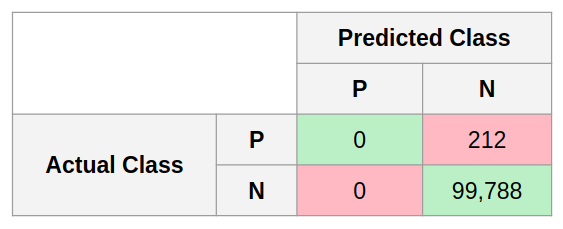
\includegraphics{../data/img/unbalanced_confusion.png}
\caption{}
\end{figure}

Even though our accuracy score (\(99.8\%\)) seems really good,
incorrectly telling 212 people they are HIV negative, is concerning.

\textbf{Our model needs to predict equally well for HIV negative and HIV
positive cases. Even if the probability of being HIV positive in Canada
is very low.}

\subsection{All predictions are equal, but some are more equal than
others}\label{all-predictions-are-equal-but-some-are-more-equal-than-others}

The only way to tell the model that it's equally important to correctly
classify the minority class (HIV+ cases) as the majority class (HIV-
cases), is to \textbf{increase the importance of correctly classifying
the minority group}.

There are multiple ways of doing this. We will be looking at the
following two methods:

\begin{itemize}
\tightlist
\item
  \textbf{Resampling data}

  \begin{itemize}
  \tightlist
  \item
    Undersampling
  \item
    Oversampling
  \end{itemize}
\item
  \textbf{Change class weights}
\end{itemize}

    \subsection{Case Study: Thoraric Surgery Survival
Rate}\label{case-study-thoraric-surgery-survival-rate}

\subsubsection{Introduction}\label{introduction}

To make our imbalanced data problem less hypothetical, let's consider
the following dataset, which can be found
\href{https://archive.ics.uci.edu/ml/datasets/Thoracic+Surgery+Data}{here}.

\emph{The data was collected retrospectively at Wroclaw Thoracic Surgery
Centre for \textbf{patients who underwent major lung resections for
primary lung cancer in the years 2007 \& 2011}. The Centre is associated
with the Department of Thoracic Surgery of the Medical University of
Wroclaw and Lower-Silesian Centre for Pulmonary Diseases, Poland, while
the research database constitutes a part of the National Lung Cancer
Registry, administered by the Institute of Tuberculosis and Pulmonary
Diseases in Warsaw, Poland.}

\textbf{Let's say we are a Life Insurance company, who's interested in
knowing whether it is a good or bad idea to insure a potential client
who will be undergoing Thoraric Surgery. If the person survives the
surgery, we want to insure the client, but if there is a high
probability of not surviving, we don't want to take the risk of insuring
the person. We have access to the potential client's patient properties
as listed below.}

\textbf{Objective:} Predict whether a person who undergoes surgery, will
be alive or dead 1 year after surgery.

\textbf{Patient Properties:}

\begin{itemize}
\tightlist
\item
  DGN: Diagnosis - specific combination of ICD-10 codes for primary and
  secondary as well multiple tumours if any
  (DGN3,DGN2,DGN4,DGN6,DGN5,DGN8,DGN1)
\item
  PRE4: Forced vital capacity - FVC (numeric)
\item
  PRE5: Volume that has been exhaled at the end of the first second of
  forced expiration - FEV1 (numeric)
\item
  PRE6: Performance status - Zubrod scale (PRZ2,PRZ1,PRZ0)
\item
  PRE7: Pain before surgery (T,F)
\item
  PRE8: Haemoptysis before surgery (T,F)
\item
  PRE9: Dyspnoea before surgery (T,F)
\item
  PRE10: Cough before surgery (T,F)
\item
  PRE11: Weakness before surgery (T,F)
\item
  PRE14: T in clinical TNM - size of the original tumour, from OC11
  (smallest) to OC14 (largest) (OC11,OC14,OC12,OC13)
\item
  PRE17: Type 2 DM - diabetes mellitus (T,F)
\item
  PRE19: MI up to 6 months (T,F)
\item
  PRE25: PAD - peripheral arterial diseases (T,F)
\item
  PRE30: Smoking (T,F)
\item
  PRE32: Asthma (T,F)
\item
  AGE: Age at surgery (numeric)
\item
  Risk1Y: 1 year survival period - (T)rue value if died (T,F)
\end{itemize}

    \subsection{Import Data}\label{import-data}

    \begin{Verbatim}[commandchars=\\\{\}]
{\color{incolor}In [{\color{incolor}307}]:} \PY{n}{data} \PY{o}{=} \PY{n}{pd}\PY{o}{.}\PY{n}{read\PYZus{}csv}\PY{p}{(}\PY{l+s+s1}{\PYZsq{}}\PY{l+s+s1}{../data/thoraric\PYZus{}surgery.csv}\PY{l+s+s1}{\PYZsq{}}\PY{p}{)}
          \PY{n}{display}\PY{p}{(}\PY{n}{data}\PY{o}{.}\PY{n}{head}\PY{p}{(}\PY{p}{)}\PY{p}{)}
          
          \PY{n}{survival\PYZus{}counts} \PY{o}{=} \PY{n}{data}\PY{o}{.}\PY{n}{Risk1Yr}\PY{o}{.}\PY{n}{value\PYZus{}counts}\PY{p}{(}\PY{p}{)}
          \PY{n+nb}{print}\PY{p}{(}\PY{l+s+s2}{\PYZdq{}}\PY{l+s+s2}{Number of patients survived: }\PY{l+s+si}{\PYZob{}\PYZcb{}}\PY{l+s+se}{\PYZbs{}n}\PY{l+s+s2}{Number of patients died: }\PY{l+s+si}{\PYZob{}\PYZcb{}}\PY{l+s+s2}{\PYZdq{}}\PY{o}{.}\PY{n}{format}\PY{p}{(}\PY{o}{*}\PY{n}{survival\PYZus{}counts}\PY{p}{)}\PY{p}{)}
\end{Verbatim}


    
    \begin{verbatim}
    DGN  PRE4  PRE5  PRE6 PRE7 PRE8 PRE9 PRE10 PRE11 PRE14 PRE17 PRE19 PRE25  \
0  DGN2  2.88  2.16  PRZ1    F    F    F     T     T  OC14     F     F     F   
1  DGN3  3.40  1.88  PRZ0    F    F    F     F     F  OC12     F     F     F   
2  DGN3  2.76  2.08  PRZ1    F    F    F     T     F  OC11     F     F     F   
3  DGN3  3.68  3.04  PRZ0    F    F    F     F     F  OC11     F     F     F   
4  DGN3  2.44  0.96  PRZ2    F    T    F     T     T  OC11     F     F     F   

  PRE30 PRE32  AGE Risk1Yr  
0     T     F   60       F  
1     T     F   51       F  
2     T     F   59       F  
3     F     F   54       F  
4     T     F   73       T  
    \end{verbatim}

    
    \begin{Verbatim}[commandchars=\\\{\}]
Number of patients survived: 400
Number of patients died: 70

    \end{Verbatim}

    \subsection{Clean and Transform Data}\label{clean-and-transform-data}

To explore the imbalanced data handling methods, we will first look at a
vanilla logistic regression model.

Our response variable is patient survival outcome (Did a patient die or
live after surgery).

This means we are working with a binary classifier.

There are two things we need to do before we can train our model:

\begin{itemize}
\tightlist
\item
  Replace strings with numbers
\item
  Change multiclass variables to binary variables
\end{itemize}

    \subsubsection{Replace strings with
numbers}\label{replace-strings-with-numbers}

We need to replace all the \texttt{"T"}'s and \texttt{"F"}'s with
\texttt{1}'s and \texttt{0}'s.

We can't use strings in a numeric equation...

    \begin{Verbatim}[commandchars=\\\{\}]
{\color{incolor}In [{\color{incolor}308}]:} \PY{n}{data}\PY{o}{.}\PY{n}{replace}\PY{p}{(}\PY{l+s+s1}{\PYZsq{}}\PY{l+s+s1}{F}\PY{l+s+s1}{\PYZsq{}}\PY{p}{,} \PY{l+m+mi}{0}\PY{p}{,} \PY{n}{inplace}\PY{o}{=}\PY{k+kc}{True}\PY{p}{)}
          \PY{n}{data}\PY{o}{.}\PY{n}{replace}\PY{p}{(}\PY{l+s+s1}{\PYZsq{}}\PY{l+s+s1}{T}\PY{l+s+s1}{\PYZsq{}}\PY{p}{,} \PY{l+m+mi}{1}\PY{p}{,} \PY{n}{inplace}\PY{o}{=}\PY{k+kc}{True}\PY{p}{)}
          \PY{n}{data}\PY{o}{.}\PY{n}{head}\PY{p}{(}\PY{p}{)}
\end{Verbatim}


\begin{Verbatim}[commandchars=\\\{\}]
{\color{outcolor}Out[{\color{outcolor}308}]:}     DGN  PRE4  PRE5  PRE6  PRE7  PRE8  PRE9  PRE10  PRE11 PRE14  PRE17  PRE19  \textbackslash{}
          0  DGN2  2.88  2.16  PRZ1     0     0     0      1      1  OC14      0      0   
          1  DGN3  3.40  1.88  PRZ0     0     0     0      0      0  OC12      0      0   
          2  DGN3  2.76  2.08  PRZ1     0     0     0      1      0  OC11      0      0   
          3  DGN3  3.68  3.04  PRZ0     0     0     0      0      0  OC11      0      0   
          4  DGN3  2.44  0.96  PRZ2     0     1     0      1      1  OC11      0      0   
          
             PRE25  PRE30  PRE32  AGE  Risk1Yr  
          0      0      1      0   60        0  
          1      0      1      0   51        0  
          2      0      1      0   59        0  
          3      0      0      0   54        0  
          4      0      1      0   73        1  
\end{Verbatim}
            
    \subsubsection{Change multiclass variables to binary
variables}\label{change-multiclass-variables-to-binary-variables}

For any model with categorical features (opposed to numeric, for
example), we need to use one-hot encoding to transform multiclass
categorical features to binary features.

For example:

\emph{DGN: Diagnosis - specific combination of ICD-10 codes for primary
and secondary as well multiple tumours if any
(DGN3,DGN2,DGN4,DGN6,DGN5,DGN8,DGN1)}

Instead of saying:

\begin{figure}
\centering
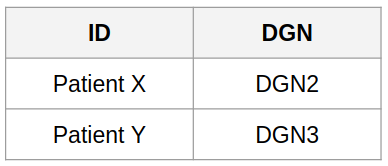
\includegraphics{../data/img/encoding_before.png}
\caption{}
\end{figure}

We need to say:

\begin{figure}
\centering
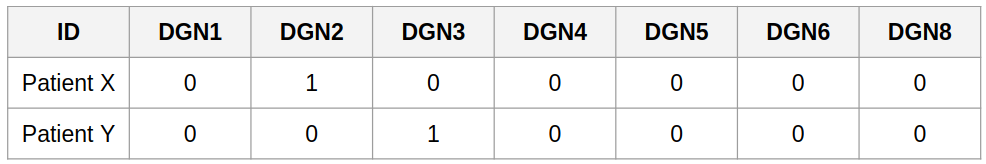
\includegraphics{../data/img/encoding_after.png}
\caption{}
\end{figure}

Don't worry too much about this. Just know that this is what is
happening below.

    \begin{Verbatim}[commandchars=\\\{\}]
{\color{incolor}In [{\color{incolor}309}]:} \PY{n}{dummy\PYZus{}cols} \PY{o}{=} \PY{p}{[}\PY{l+s+s1}{\PYZsq{}}\PY{l+s+s1}{DGN}\PY{l+s+s1}{\PYZsq{}}\PY{p}{,} \PY{l+s+s1}{\PYZsq{}}\PY{l+s+s1}{PRE6}\PY{l+s+s1}{\PYZsq{}}\PY{p}{,} \PY{l+s+s1}{\PYZsq{}}\PY{l+s+s1}{PRE14}\PY{l+s+s1}{\PYZsq{}}\PY{p}{]}
          \PY{n}{dummies} \PY{o}{=} \PY{n}{pd}\PY{o}{.}\PY{n}{get\PYZus{}dummies}\PY{p}{(}\PY{n}{data}\PY{p}{[}\PY{n}{dummy\PYZus{}cols}\PY{p}{]}\PY{p}{)}
          
          \PY{n}{data} \PY{o}{=} \PY{n}{data}\PY{o}{.}\PY{n}{join}\PY{p}{(}\PY{n}{dummies}\PY{p}{)}
          \PY{n}{data}\PY{o}{.}\PY{n}{drop}\PY{p}{(}\PY{n}{columns}\PY{o}{=}\PY{n}{dummy\PYZus{}cols}\PY{p}{,} \PY{n}{inplace}\PY{o}{=}\PY{k+kc}{True}\PY{p}{)}
          \PY{n}{data}\PY{o}{.}\PY{n}{head}\PY{p}{(}\PY{p}{)}
          
          \PY{c+c1}{\PYZsh{} split into train and test data}
          
          \PY{c+c1}{\PYZsh{} patient features}
          \PY{n}{X} \PY{o}{=} \PY{n}{data}\PY{o}{.}\PY{n}{loc}\PY{p}{[}\PY{p}{:}\PY{p}{,} \PY{n}{data}\PY{o}{.}\PY{n}{columns}\PY{o}{!=}\PY{l+s+s1}{\PYZsq{}}\PY{l+s+s1}{Risk1Yr}\PY{l+s+s1}{\PYZsq{}}\PY{p}{]}
          \PY{c+c1}{\PYZsh{} response variable (what we want to predict)}
          \PY{n}{y} \PY{o}{=} \PY{n}{data}\PY{p}{[}\PY{l+s+s1}{\PYZsq{}}\PY{l+s+s1}{Risk1Yr}\PY{l+s+s1}{\PYZsq{}}\PY{p}{]}
          
          \PY{c+c1}{\PYZsh{} split the data into training and testing (70\PYZpc{} of the data used for training, and 30\PYZpc{} used for testing)}
          \PY{c+c1}{\PYZsh{} X\PYZus{}train, X\PYZus{}test, y\PYZus{}train, y\PYZus{}test = train\PYZus{}test\PYZus{}split(X, y, test\PYZus{}size=0.3, random\PYZus{}state=1234)}
          \PY{n}{data\PYZus{}train}\PY{p}{,} \PY{n}{data\PYZus{}test} \PY{o}{=} \PY{n}{train\PYZus{}test\PYZus{}split}\PY{p}{(}\PY{n}{data}\PY{p}{,} \PY{n}{test\PYZus{}size}\PY{o}{=}\PY{l+m+mf}{0.3}\PY{p}{,} \PY{n}{random\PYZus{}state}\PY{o}{=}\PY{l+m+mi}{1234}\PY{p}{)}
          
          \PY{c+c1}{\PYZsh{} we will be using the same test dataset, but change the train dataset as we go}
          \PY{n}{X\PYZus{}test} \PY{o}{=} \PY{n}{data\PYZus{}test}\PY{o}{.}\PY{n}{loc}\PY{p}{[}\PY{p}{:}\PY{p}{,} \PY{n}{data}\PY{o}{.}\PY{n}{columns}\PY{o}{!=}\PY{l+s+s1}{\PYZsq{}}\PY{l+s+s1}{Risk1Yr}\PY{l+s+s1}{\PYZsq{}}\PY{p}{]}
          \PY{n}{y\PYZus{}test} \PY{o}{=} \PY{n}{data\PYZus{}test}\PY{p}{[}\PY{l+s+s1}{\PYZsq{}}\PY{l+s+s1}{Risk1Yr}\PY{l+s+s1}{\PYZsq{}}\PY{p}{]}
\end{Verbatim}


    \subsection{Vanilla Logistic Regression with data
as-is}\label{vanilla-logistic-regression-with-data-as-is}

As we saw above, the vast majority of patients survived (\(400\) out of
\(470\) patients) the surgery.

If we want the model to maximize the correct number of predictions(in
other words, we do not attach more importance to correctly classifying a
specific class), we can use train the logistic regression model on the
data as-is.

    \begin{Verbatim}[commandchars=\\\{\}]
{\color{incolor}In [{\color{incolor}310}]:} \PY{c+c1}{\PYZsh{} initialize score dict}
          \PY{n}{scores} \PY{o}{=} \PY{p}{\PYZob{}}\PY{p}{\PYZcb{}}
          
          \PY{c+c1}{\PYZsh{} \PYZsh{} patient features}
          \PY{c+c1}{\PYZsh{} X = data.loc[:, data.columns!=\PYZsq{}Risk1Yr\PYZsq{}]}
          \PY{c+c1}{\PYZsh{} \PYZsh{} response variable (what we want to predict)}
          \PY{c+c1}{\PYZsh{} y = data[\PYZsq{}Risk1Yr\PYZsq{}]}
          
          \PY{c+c1}{\PYZsh{} \PYZsh{} split the data into training and testing (70\PYZpc{} of the data used for training, and 30\PYZpc{} used for testing)}
          \PY{c+c1}{\PYZsh{} X\PYZus{}train, X\PYZus{}test, y\PYZus{}train, y\PYZus{}test = train\PYZus{}test\PYZus{}split(X, y, test\PYZus{}size=0.3, random\PYZus{}state=1234)}
          \PY{n}{X\PYZus{}train} \PY{o}{=} \PY{n}{data\PYZus{}train}\PY{o}{.}\PY{n}{loc}\PY{p}{[}\PY{p}{:}\PY{p}{,} \PY{n}{data\PYZus{}train}\PY{o}{.}\PY{n}{columns}\PY{o}{!=}\PY{l+s+s1}{\PYZsq{}}\PY{l+s+s1}{Risk1Yr}\PY{l+s+s1}{\PYZsq{}}\PY{p}{]}
          \PY{n}{y\PYZus{}train} \PY{o}{=} \PY{n}{data\PYZus{}train}\PY{p}{[}\PY{l+s+s1}{\PYZsq{}}\PY{l+s+s1}{Risk1Yr}\PY{l+s+s1}{\PYZsq{}}\PY{p}{]}
          
          
          \PY{c+c1}{\PYZsh{} train the model}
          \PY{n}{lr} \PY{o}{=} \PY{n}{LogisticRegression}\PY{p}{(}\PY{p}{)}
          \PY{n}{lr}\PY{o}{.}\PY{n}{fit}\PY{p}{(}\PY{n}{X}\PY{o}{=}\PY{n}{X\PYZus{}train}\PY{p}{,} \PY{n}{y} \PY{o}{=} \PY{n}{y\PYZus{}train}\PY{p}{)}
          
          \PY{c+c1}{\PYZsh{} test the model on unseen test data}
          \PY{n}{predictions} \PY{o}{=} \PY{n}{lr}\PY{o}{.}\PY{n}{predict}\PY{p}{(}\PY{n}{X\PYZus{}test}\PY{p}{)}
          
          \PY{n}{conf\PYZus{}mat} \PY{o}{=} \PY{n}{confusion\PYZus{}matrix}\PY{p}{(}\PY{n}{y\PYZus{}true}\PY{o}{=}\PY{n}{y\PYZus{}test}\PY{p}{,} \PY{n}{y\PYZus{}pred}\PY{o}{=}\PY{n}{predictions}\PY{p}{)}
          \PY{n}{test\PYZus{}accuracy} \PY{o}{=} \PY{p}{(}\PY{n}{conf\PYZus{}mat}\PY{p}{[}\PY{l+m+mi}{0}\PY{p}{,} \PY{l+m+mi}{0}\PY{p}{]} \PY{o}{+} \PY{n}{conf\PYZus{}mat}\PY{p}{[}\PY{l+m+mi}{1}\PY{p}{,} \PY{l+m+mi}{1}\PY{p}{]}\PY{p}{)} \PY{o}{/} \PY{n}{np}\PY{o}{.}\PY{n}{sum}\PY{p}{(}\PY{n}{conf\PYZus{}mat}\PY{p}{)}
          
          \PY{c+c1}{\PYZsh{} store scores for later}
          \PY{n}{scores}\PY{p}{[}\PY{l+s+s1}{\PYZsq{}}\PY{l+s+s1}{vanilla}\PY{l+s+s1}{\PYZsq{}}\PY{p}{]} \PY{o}{=} \PY{n}{precision\PYZus{}recall\PYZus{}fscore\PYZus{}support}\PY{p}{(}\PY{n}{y\PYZus{}true}\PY{o}{=}\PY{n}{y\PYZus{}test}\PY{p}{,} \PY{n}{y\PYZus{}pred}\PY{o}{=}\PY{n}{predictions}\PY{p}{,} \PY{n}{average}\PY{o}{=}\PY{l+s+s1}{\PYZsq{}}\PY{l+s+s1}{binary}\PY{l+s+s1}{\PYZsq{}}\PY{p}{)}
          
          \PY{n+nb}{print}\PY{p}{(}\PY{l+s+s1}{\PYZsq{}}\PY{l+s+s1}{Accuracy: }\PY{l+s+si}{\PYZob{}0:.2f\PYZcb{}}\PY{l+s+s1}{\PYZpc{}}\PY{l+s+s1}{\PYZsq{}}\PY{o}{.}\PY{n}{format}\PY{p}{(}\PY{n}{test\PYZus{}accuracy}\PY{o}{*}\PY{l+m+mi}{100}\PY{p}{)}\PY{p}{)}
\end{Verbatim}


    \begin{Verbatim}[commandchars=\\\{\}]
Accuracy: 81.56\%

    \end{Verbatim}

    So in terms of \emph{number of correct predictions}, our model seems to
be doing quite well.

Let's take a look at the confusion matrix, which will reveal a bit more
about how our model does its classifications.

    \begin{Verbatim}[commandchars=\\\{\}]
{\color{incolor}In [{\color{incolor}311}]:} \PY{n}{pd}\PY{o}{.}\PY{n}{DataFrame}\PY{p}{(}\PY{n}{conf\PYZus{}mat}\PY{p}{,} \PY{n}{index}\PY{o}{=}\PY{p}{[}\PY{l+s+s1}{\PYZsq{}}\PY{l+s+s1}{Actual\PYZus{}Survived}\PY{l+s+s1}{\PYZsq{}}\PY{p}{,} \PY{l+s+s1}{\PYZsq{}}\PY{l+s+s1}{Actual\PYZus{}Died}\PY{l+s+s1}{\PYZsq{}}\PY{p}{]}\PY{p}{,} \PY{n}{columns}\PY{o}{=}\PY{p}{[}\PY{l+s+s1}{\PYZsq{}}\PY{l+s+s1}{Predicted\PYZus{}Survived}\PY{l+s+s1}{\PYZsq{}}\PY{p}{,} \PY{l+s+s1}{\PYZsq{}}\PY{l+s+s1}{Predicted\PYZus{}Died}\PY{l+s+s1}{\PYZsq{}}\PY{p}{]}\PY{p}{)}
\end{Verbatim}


\begin{Verbatim}[commandchars=\\\{\}]
{\color{outcolor}Out[{\color{outcolor}311}]:}                  Predicted\_Survived  Predicted\_Died
          Actual\_Survived                 114               2
          Actual\_Died                      24               1
\end{Verbatim}
            
    The confusion matrix is showing that our model rarely ever predict that
a patient will die. Since it's a safer bet to predict that a patient has
survived (due to the imbalance), the model choses to do this when there
is a certain level of uncertainty.

However, we want to make sure that our potential client is going to
survive. Even though survival is more likely, if our patient has the
properties similar to the small proportion of patients who typically do
not survive, we want to know about it.

    \subsection{Method 1: Resampling Data}\label{method-1-resampling-data}

\subsubsection{Undersampling}\label{undersampling}

Undersampling is the process of \textbf{reducing the number of samples
of the majority class} during model training.

We aim to end up with a reduced number of majority class samples equal
to the number of samples in the minority class.

This will result in balanced data and cause the model to pay more
attention to the minority class (since it now has just as many samples
as the majority class).

    \begin{Verbatim}[commandchars=\\\{\}]
{\color{incolor}In [{\color{incolor}312}]:} \PY{c+c1}{\PYZsh{} determine the number of samples in the minority class}
          \PY{n}{label\PYZus{}min\PYZus{}count} \PY{o}{=} \PY{n}{data\PYZus{}train}\PY{o}{.}\PY{n}{Risk1Yr}\PY{o}{.}\PY{n}{value\PYZus{}counts}\PY{p}{(}\PY{p}{)}\PY{o}{.}\PY{n}{min}\PY{p}{(}\PY{p}{)}
          \PY{c+c1}{\PYZsh{} determine the label of the minority class}
          \PY{n}{label\PYZus{}min} \PY{o}{=} \PY{n}{data\PYZus{}train}\PY{o}{.}\PY{n}{Risk1Yr}\PY{o}{.}\PY{n}{value\PYZus{}counts}\PY{p}{(}\PY{p}{)}\PY{o}{.}\PY{n}{idxmin}\PY{p}{(}\PY{p}{)}
          
          \PY{c+c1}{\PYZsh{} create data subsets for the 2 classes}
          \PY{n}{data\PYZus{}max\PYZus{}label} \PY{o}{=} \PY{n}{data\PYZus{}train}\PY{p}{[}\PY{n}{data\PYZus{}train}\PY{o}{.}\PY{n}{Risk1Yr} \PY{o}{!=} \PY{n}{label\PYZus{}min}\PY{p}{]}
          \PY{n}{data\PYZus{}min\PYZus{}label} \PY{o}{=} \PY{n}{data\PYZus{}train}\PY{p}{[}\PY{n}{data\PYZus{}train}\PY{o}{.}\PY{n}{Risk1Yr} \PY{o}{==} \PY{n}{label\PYZus{}min}\PY{p}{]}
          
          \PY{c+c1}{\PYZsh{} reduce the number of samples in the majority class subset}
          \PY{n}{data\PYZus{}max\PYZus{}downsample} \PY{o}{=} \PY{n}{data\PYZus{}max\PYZus{}label}\PY{o}{.}\PY{n}{sample}\PY{p}{(}\PY{n}{n} \PY{o}{=} \PY{n}{label\PYZus{}min\PYZus{}count}\PY{p}{,} \PY{n}{replace}\PY{o}{=}\PY{k+kc}{False}\PY{p}{,} \PY{n}{random\PYZus{}state}\PY{o}{=}\PY{l+m+mi}{1234}\PY{p}{)}
          
          \PY{c+c1}{\PYZsh{} merge the two subsets to give us the balanced dataset}
          \PY{n}{data\PYZus{}balanced} \PY{o}{=} \PY{n}{data\PYZus{}min\PYZus{}label}\PY{o}{.}\PY{n}{append}\PY{p}{(}\PY{n}{data\PYZus{}max\PYZus{}downsample}\PY{p}{)}
          
          \PY{n}{survival\PYZus{}counts} \PY{o}{=} \PY{n}{data\PYZus{}train}\PY{o}{.}\PY{n}{Risk1Yr}\PY{o}{.}\PY{n}{value\PYZus{}counts}\PY{p}{(}\PY{p}{)}
          \PY{n+nb}{print}\PY{p}{(}\PY{l+s+s2}{\PYZdq{}}\PY{l+s+s2}{Original Data:}\PY{l+s+se}{\PYZbs{}n}\PY{l+s+s2}{Number of patients survived: }\PY{l+s+si}{\PYZob{}\PYZcb{}}\PY{l+s+se}{\PYZbs{}n}\PY{l+s+s2}{Number of patients died: }\PY{l+s+si}{\PYZob{}\PYZcb{}}\PY{l+s+se}{\PYZbs{}n}\PY{l+s+s2}{\PYZdq{}}\PY{o}{.}\PY{n}{format}\PY{p}{(}\PY{o}{*}\PY{n}{survival\PYZus{}counts}\PY{p}{)}\PY{p}{)}
          
          \PY{n}{survival\PYZus{}counts} \PY{o}{=} \PY{n}{data\PYZus{}balanced}\PY{o}{.}\PY{n}{Risk1Yr}\PY{o}{.}\PY{n}{value\PYZus{}counts}\PY{p}{(}\PY{p}{)}
          \PY{n+nb}{print}\PY{p}{(}\PY{l+s+s2}{\PYZdq{}}\PY{l+s+s2}{Undersampled, Balanced Data:}\PY{l+s+se}{\PYZbs{}n}\PY{l+s+s2}{Number of patients survived: }\PY{l+s+si}{\PYZob{}\PYZcb{}}\PY{l+s+se}{\PYZbs{}n}\PY{l+s+s2}{Number of patients died: }\PY{l+s+si}{\PYZob{}\PYZcb{}}\PY{l+s+s2}{\PYZdq{}}\PY{o}{.}\PY{n}{format}\PY{p}{(}\PY{o}{*}\PY{n}{survival\PYZus{}counts}\PY{p}{)}\PY{p}{)}
\end{Verbatim}


    \begin{Verbatim}[commandchars=\\\{\}]
Original Data:
Number of patients survived: 284
Number of patients died: 45

Undersampled, Balanced Data:
Number of patients survived: 45
Number of patients died: 45

    \end{Verbatim}

    \begin{Verbatim}[commandchars=\\\{\}]
{\color{incolor}In [{\color{incolor}313}]:} \PY{c+c1}{\PYZsh{} patient features}
          \PY{n}{X\PYZus{}train} \PY{o}{=} \PY{n}{data\PYZus{}balanced}\PY{o}{.}\PY{n}{loc}\PY{p}{[}\PY{p}{:}\PY{p}{,} \PY{n}{data\PYZus{}balanced}\PY{o}{.}\PY{n}{columns}\PY{o}{!=}\PY{l+s+s1}{\PYZsq{}}\PY{l+s+s1}{Risk1Yr}\PY{l+s+s1}{\PYZsq{}}\PY{p}{]}
          \PY{c+c1}{\PYZsh{} response variable (what we want to predict)}
          \PY{n}{y\PYZus{}train} \PY{o}{=} \PY{n}{data\PYZus{}balanced}\PY{p}{[}\PY{l+s+s1}{\PYZsq{}}\PY{l+s+s1}{Risk1Yr}\PY{l+s+s1}{\PYZsq{}}\PY{p}{]}
          
          \PY{c+c1}{\PYZsh{} split the data into training and testing (70\PYZpc{} of the data used for training, and 30\PYZpc{} used for testing)}
          \PY{c+c1}{\PYZsh{} X\PYZus{}train, X\PYZus{}test, y\PYZus{}train, y\PYZus{}test = train\PYZus{}test\PYZus{}split(X, y, test\PYZus{}size=0.3, random\PYZus{}state=1234)}
          \PY{c+c1}{\PYZsh{} }
          
          \PY{c+c1}{\PYZsh{} train the model}
          \PY{n}{lr} \PY{o}{=} \PY{n}{LogisticRegression}\PY{p}{(}\PY{p}{)}
          \PY{n}{lr}\PY{o}{.}\PY{n}{fit}\PY{p}{(}\PY{n}{X}\PY{o}{=}\PY{n}{X\PYZus{}train}\PY{p}{,} \PY{n}{y} \PY{o}{=} \PY{n}{y\PYZus{}train}\PY{p}{)}
          
          \PY{c+c1}{\PYZsh{} test the model on unseen test data}
          \PY{n}{predictions} \PY{o}{=} \PY{n}{lr}\PY{o}{.}\PY{n}{predict}\PY{p}{(}\PY{n}{X\PYZus{}test}\PY{p}{)}
          
          \PY{n}{conf\PYZus{}mat} \PY{o}{=} \PY{n}{confusion\PYZus{}matrix}\PY{p}{(}\PY{n}{y\PYZus{}true}\PY{o}{=}\PY{n}{y\PYZus{}test}\PY{p}{,} \PY{n}{y\PYZus{}pred}\PY{o}{=}\PY{n}{predictions}\PY{p}{)}
          \PY{n}{test\PYZus{}accuracy} \PY{o}{=} \PY{p}{(}\PY{n}{conf\PYZus{}mat}\PY{p}{[}\PY{l+m+mi}{0}\PY{p}{,} \PY{l+m+mi}{0}\PY{p}{]} \PY{o}{+} \PY{n}{conf\PYZus{}mat}\PY{p}{[}\PY{l+m+mi}{1}\PY{p}{,} \PY{l+m+mi}{1}\PY{p}{]}\PY{p}{)} \PY{o}{/} \PY{n}{np}\PY{o}{.}\PY{n}{sum}\PY{p}{(}\PY{n}{conf\PYZus{}mat}\PY{p}{)}
          
          \PY{c+c1}{\PYZsh{} store scores for later}
          \PY{n}{scores}\PY{p}{[}\PY{l+s+s1}{\PYZsq{}}\PY{l+s+s1}{undersampling}\PY{l+s+s1}{\PYZsq{}}\PY{p}{]} \PY{o}{=} \PY{n}{precision\PYZus{}recall\PYZus{}fscore\PYZus{}support}\PY{p}{(}\PY{n}{y\PYZus{}true}\PY{o}{=}\PY{n}{y\PYZus{}test}\PY{p}{,} \PY{n}{y\PYZus{}pred}\PY{o}{=}\PY{n}{predictions}\PY{p}{,} \PY{n}{average}\PY{o}{=}\PY{l+s+s1}{\PYZsq{}}\PY{l+s+s1}{binary}\PY{l+s+s1}{\PYZsq{}}\PY{p}{)}
          
          \PY{n+nb}{print}\PY{p}{(}\PY{l+s+s1}{\PYZsq{}}\PY{l+s+s1}{Accuracy: }\PY{l+s+si}{\PYZob{}0:.2f\PYZcb{}}\PY{l+s+s1}{\PYZpc{}}\PY{l+s+s1}{\PYZsq{}}\PY{o}{.}\PY{n}{format}\PY{p}{(}\PY{n}{test\PYZus{}accuracy}\PY{o}{*}\PY{l+m+mi}{100}\PY{p}{)}\PY{p}{)}
\end{Verbatim}


    \begin{Verbatim}[commandchars=\\\{\}]
Accuracy: 60.99\%

    \end{Verbatim}

    \begin{Verbatim}[commandchars=\\\{\}]
{\color{incolor}In [{\color{incolor}314}]:} \PY{n}{pd}\PY{o}{.}\PY{n}{DataFrame}\PY{p}{(}\PY{n}{conf\PYZus{}mat}\PY{p}{,} \PY{n}{index}\PY{o}{=}\PY{p}{[}\PY{l+s+s1}{\PYZsq{}}\PY{l+s+s1}{Actual\PYZus{}Survived}\PY{l+s+s1}{\PYZsq{}}\PY{p}{,} \PY{l+s+s1}{\PYZsq{}}\PY{l+s+s1}{Actual\PYZus{}Died}\PY{l+s+s1}{\PYZsq{}}\PY{p}{]}\PY{p}{,} \PY{n}{columns}\PY{o}{=}\PY{p}{[}\PY{l+s+s1}{\PYZsq{}}\PY{l+s+s1}{Predicted\PYZus{}Survived}\PY{l+s+s1}{\PYZsq{}}\PY{p}{,} \PY{l+s+s1}{\PYZsq{}}\PY{l+s+s1}{Predicted\PYZus{}Died}\PY{l+s+s1}{\PYZsq{}}\PY{p}{]}\PY{p}{)}
\end{Verbatim}


\begin{Verbatim}[commandchars=\\\{\}]
{\color{outcolor}Out[{\color{outcolor}314}]:}                  Predicted\_Survived  Predicted\_Died
          Actual\_Survived                  73              43
          Actual\_Died                      12              13
\end{Verbatim}
            
    We can see that our results are more balanced, but our overall number of
correct predictions has decreased quite a bit.

One of the main issues here, is that we lost a lot of training data by
undersampling. Since we didn't have many samples to start off with, we
end up with a small training dataset.

For this reason, it makes more sense to oversample, rather than
undersample.

    \subsubsection{Oversampling}\label{oversampling}

Oversampling is the process of \textbf{increasing the number of samples
of the minority class} during model training.

We aim to end up with a increased number of minority class samples equal
to the number of samples in the majority class.

This will result in balanced data and cause the model to pay more
attention to the minority class (since it now has just as many samples
as the majority class), while still using all the data we have
available.

    \begin{Verbatim}[commandchars=\\\{\}]
{\color{incolor}In [{\color{incolor}315}]:} \PY{c+c1}{\PYZsh{} determine the  number of samples in the majority class}
          \PY{c+c1}{\PYZsh{} y = data\PYZus{}train[\PYZsq{}Risk1Yr\PYZsq{}]}
          \PY{n}{label\PYZus{}max\PYZus{}count} \PY{o}{=} \PY{n}{data\PYZus{}train}\PY{o}{.}\PY{n}{Risk1Yr}\PY{o}{.}\PY{n}{value\PYZus{}counts}\PY{p}{(}\PY{p}{)}\PY{o}{.}\PY{n}{max}\PY{p}{(}\PY{p}{)}
          \PY{c+c1}{\PYZsh{} determine the label of the majority class}
          \PY{n}{label\PYZus{}max} \PY{o}{=} \PY{n}{data\PYZus{}train}\PY{o}{.}\PY{n}{Risk1Yr}\PY{o}{.}\PY{n}{value\PYZus{}counts}\PY{p}{(}\PY{p}{)}\PY{o}{.}\PY{n}{idxmax}\PY{p}{(}\PY{p}{)}
          
          \PY{c+c1}{\PYZsh{} increase the number of samples in the minority class subset}
          \PY{n}{data\PYZus{}min\PYZus{}upsample} \PY{o}{=} \PY{n}{data\PYZus{}min\PYZus{}label}\PY{o}{.}\PY{n}{sample}\PY{p}{(}\PY{n}{n} \PY{o}{=} \PY{n}{label\PYZus{}max\PYZus{}count}\PY{p}{,} \PY{n}{replace}\PY{o}{=}\PY{k+kc}{True}\PY{p}{,} \PY{n}{random\PYZus{}state}\PY{o}{=}\PY{l+m+mi}{1234}\PY{p}{)}
          
          \PY{c+c1}{\PYZsh{} merge the two subsets to give us the balanced dataset}
          \PY{n}{data\PYZus{}balanced} \PY{o}{=} \PY{n}{data\PYZus{}max\PYZus{}label}\PY{o}{.}\PY{n}{append}\PY{p}{(}\PY{n}{data\PYZus{}min\PYZus{}upsample}\PY{p}{)}
          
          \PY{n}{survival\PYZus{}counts} \PY{o}{=} \PY{n}{data\PYZus{}train}\PY{o}{.}\PY{n}{Risk1Yr}\PY{o}{.}\PY{n}{value\PYZus{}counts}\PY{p}{(}\PY{p}{)}
          \PY{n+nb}{print}\PY{p}{(}\PY{l+s+s2}{\PYZdq{}}\PY{l+s+s2}{Original Data:}\PY{l+s+se}{\PYZbs{}n}\PY{l+s+s2}{Number of patients survived: }\PY{l+s+si}{\PYZob{}\PYZcb{}}\PY{l+s+se}{\PYZbs{}n}\PY{l+s+s2}{Number of patients died: }\PY{l+s+si}{\PYZob{}\PYZcb{}}\PY{l+s+se}{\PYZbs{}n}\PY{l+s+s2}{\PYZdq{}}\PY{o}{.}\PY{n}{format}\PY{p}{(}\PY{o}{*}\PY{n}{survival\PYZus{}counts}\PY{p}{)}\PY{p}{)}
          
          \PY{n}{survival\PYZus{}counts} \PY{o}{=} \PY{n}{data\PYZus{}balanced}\PY{o}{.}\PY{n}{Risk1Yr}\PY{o}{.}\PY{n}{value\PYZus{}counts}\PY{p}{(}\PY{p}{)}
          \PY{n+nb}{print}\PY{p}{(}\PY{l+s+s2}{\PYZdq{}}\PY{l+s+s2}{Oversampled, Balanced Data:}\PY{l+s+se}{\PYZbs{}n}\PY{l+s+s2}{Number of patients survived: }\PY{l+s+si}{\PYZob{}\PYZcb{}}\PY{l+s+se}{\PYZbs{}n}\PY{l+s+s2}{Number of patients died: }\PY{l+s+si}{\PYZob{}\PYZcb{}}\PY{l+s+s2}{\PYZdq{}}\PY{o}{.}\PY{n}{format}\PY{p}{(}\PY{o}{*}\PY{n}{survival\PYZus{}counts}\PY{p}{)}\PY{p}{)}
\end{Verbatim}


    \begin{Verbatim}[commandchars=\\\{\}]
Original Data:
Number of patients survived: 284
Number of patients died: 45

Oversampled, Balanced Data:
Number of patients survived: 284
Number of patients died: 284

    \end{Verbatim}

    \begin{Verbatim}[commandchars=\\\{\}]
{\color{incolor}In [{\color{incolor}316}]:} \PY{c+c1}{\PYZsh{} patient features}
          \PY{n}{X\PYZus{}train} \PY{o}{=} \PY{n}{data\PYZus{}balanced}\PY{o}{.}\PY{n}{loc}\PY{p}{[}\PY{p}{:}\PY{p}{,} \PY{n}{data\PYZus{}balanced}\PY{o}{.}\PY{n}{columns}\PY{o}{!=}\PY{l+s+s1}{\PYZsq{}}\PY{l+s+s1}{Risk1Yr}\PY{l+s+s1}{\PYZsq{}}\PY{p}{]}
          \PY{c+c1}{\PYZsh{} response variable (what we want to predict)}
          \PY{n}{y\PYZus{}train} \PY{o}{=} \PY{n}{data\PYZus{}balanced}\PY{p}{[}\PY{l+s+s1}{\PYZsq{}}\PY{l+s+s1}{Risk1Yr}\PY{l+s+s1}{\PYZsq{}}\PY{p}{]}
          
          \PY{c+c1}{\PYZsh{} split the data into training and testing (70\PYZpc{} of the data used for trainning, and 30\PYZpc{} used for testing)}
          \PY{c+c1}{\PYZsh{} X\PYZus{}train, X\PYZus{}test, y\PYZus{}train, y\PYZus{}test = train\PYZus{}test\PYZus{}split(X, y, test\PYZus{}size=0.3, random\PYZus{}state=1234)}
          \PY{c+c1}{\PYZsh{} }
          
          \PY{c+c1}{\PYZsh{} train the model}
          \PY{n}{lr} \PY{o}{=} \PY{n}{LogisticRegression}\PY{p}{(}\PY{p}{)}
          \PY{n}{lr}\PY{o}{.}\PY{n}{fit}\PY{p}{(}\PY{n}{X}\PY{o}{=}\PY{n}{X\PYZus{}train}\PY{p}{,} \PY{n}{y} \PY{o}{=} \PY{n}{y\PYZus{}train}\PY{p}{)}
          
          \PY{c+c1}{\PYZsh{} test the model on unseen test data}
          \PY{n}{predictions} \PY{o}{=} \PY{n}{lr}\PY{o}{.}\PY{n}{predict}\PY{p}{(}\PY{n}{X\PYZus{}test}\PY{p}{)}
          
          \PY{n}{conf\PYZus{}mat} \PY{o}{=} \PY{n}{confusion\PYZus{}matrix}\PY{p}{(}\PY{n}{y\PYZus{}true}\PY{o}{=}\PY{n}{y\PYZus{}test}\PY{p}{,} \PY{n}{y\PYZus{}pred}\PY{o}{=}\PY{n}{predictions}\PY{p}{)}
          \PY{n}{test\PYZus{}accuracy} \PY{o}{=} \PY{p}{(}\PY{n}{conf\PYZus{}mat}\PY{p}{[}\PY{l+m+mi}{0}\PY{p}{,} \PY{l+m+mi}{0}\PY{p}{]} \PY{o}{+} \PY{n}{conf\PYZus{}mat}\PY{p}{[}\PY{l+m+mi}{1}\PY{p}{,} \PY{l+m+mi}{1}\PY{p}{]}\PY{p}{)} \PY{o}{/} \PY{n}{np}\PY{o}{.}\PY{n}{sum}\PY{p}{(}\PY{n}{conf\PYZus{}mat}\PY{p}{)}
          
          \PY{c+c1}{\PYZsh{} store scores for later}
          \PY{n}{scores}\PY{p}{[}\PY{l+s+s1}{\PYZsq{}}\PY{l+s+s1}{oversampling}\PY{l+s+s1}{\PYZsq{}}\PY{p}{]} \PY{o}{=} \PY{n}{precision\PYZus{}recall\PYZus{}fscore\PYZus{}support}\PY{p}{(}\PY{n}{y\PYZus{}true}\PY{o}{=}\PY{n}{y\PYZus{}test}\PY{p}{,} \PY{n}{y\PYZus{}pred}\PY{o}{=}\PY{n}{predictions}\PY{p}{,} \PY{n}{average}\PY{o}{=}\PY{l+s+s1}{\PYZsq{}}\PY{l+s+s1}{binary}\PY{l+s+s1}{\PYZsq{}}\PY{p}{)}
          
          \PY{n+nb}{print}\PY{p}{(}\PY{l+s+s1}{\PYZsq{}}\PY{l+s+s1}{Accuracy: }\PY{l+s+si}{\PYZob{}0:.2f\PYZcb{}}\PY{l+s+s1}{\PYZpc{}}\PY{l+s+s1}{\PYZsq{}}\PY{o}{.}\PY{n}{format}\PY{p}{(}\PY{n}{test\PYZus{}accuracy}\PY{o}{*}\PY{l+m+mi}{100}\PY{p}{)}\PY{p}{)}
\end{Verbatim}


    \begin{Verbatim}[commandchars=\\\{\}]
Accuracy: 68.79\%

    \end{Verbatim}

    \begin{Verbatim}[commandchars=\\\{\}]
{\color{incolor}In [{\color{incolor}317}]:} \PY{n}{pd}\PY{o}{.}\PY{n}{DataFrame}\PY{p}{(}\PY{n}{conf\PYZus{}mat}\PY{p}{,} \PY{n}{index}\PY{o}{=}\PY{p}{[}\PY{l+s+s1}{\PYZsq{}}\PY{l+s+s1}{Actual\PYZus{}Survived}\PY{l+s+s1}{\PYZsq{}}\PY{p}{,} \PY{l+s+s1}{\PYZsq{}}\PY{l+s+s1}{Actual\PYZus{}Died}\PY{l+s+s1}{\PYZsq{}}\PY{p}{]}\PY{p}{,} \PY{n}{columns}\PY{o}{=}\PY{p}{[}\PY{l+s+s1}{\PYZsq{}}\PY{l+s+s1}{Predicted\PYZus{}Survived}\PY{l+s+s1}{\PYZsq{}}\PY{p}{,} \PY{l+s+s1}{\PYZsq{}}\PY{l+s+s1}{Predicted\PYZus{}Died}\PY{l+s+s1}{\PYZsq{}}\PY{p}{]}\PY{p}{)}
\end{Verbatim}


\begin{Verbatim}[commandchars=\\\{\}]
{\color{outcolor}Out[{\color{outcolor}317}]:}                  Predicted\_Survived  Predicted\_Died
          Actual\_Survived                  83              33
          Actual\_Died                      11              14
\end{Verbatim}
            
    \subsection{Method 2: Change Class
Weights}\label{method-2-change-class-weights}

    \begin{Verbatim}[commandchars=\\\{\}]
{\color{incolor}In [{\color{incolor}318}]:} \PY{c+c1}{\PYZsh{} \PYZsh{} patient features}
          \PY{c+c1}{\PYZsh{} X = data.loc[:, data.columns!=\PYZsq{}Risk1Yr\PYZsq{}]}
          \PY{c+c1}{\PYZsh{} \PYZsh{} response variable (what we want to predict)}
          \PY{c+c1}{\PYZsh{} y = data[\PYZsq{}Risk1Yr\PYZsq{}]}
          
          \PY{c+c1}{\PYZsh{} \PYZsh{} split the data into training and testing (70\PYZpc{} of the data used for training, and 30\PYZpc{} used for testing)}
          \PY{c+c1}{\PYZsh{} X\PYZus{}train, X\PYZus{}test, y\PYZus{}train, y\PYZus{}test = train\PYZus{}test\PYZus{}split(X, y, test\PYZus{}size=0.3, random\PYZus{}state=1234)}
          
          \PY{n}{X\PYZus{}train} \PY{o}{=} \PY{n}{data\PYZus{}train}\PY{o}{.}\PY{n}{loc}\PY{p}{[}\PY{p}{:}\PY{p}{,} \PY{n}{data\PYZus{}train}\PY{o}{.}\PY{n}{columns}\PY{o}{!=}\PY{l+s+s1}{\PYZsq{}}\PY{l+s+s1}{Risk1Yr}\PY{l+s+s1}{\PYZsq{}}\PY{p}{]}
          \PY{n}{y\PYZus{}train} \PY{o}{=} \PY{n}{data\PYZus{}train}\PY{p}{[}\PY{l+s+s1}{\PYZsq{}}\PY{l+s+s1}{Risk1Yr}\PY{l+s+s1}{\PYZsq{}}\PY{p}{]}
          
          \PY{c+c1}{\PYZsh{} train the model}
          \PY{n}{lr} \PY{o}{=} \PY{n}{LogisticRegression}\PY{p}{(}\PY{n}{class\PYZus{}weight}\PY{o}{=}\PY{l+s+s1}{\PYZsq{}}\PY{l+s+s1}{balanced}\PY{l+s+s1}{\PYZsq{}}\PY{p}{)}
          \PY{n}{lr}\PY{o}{.}\PY{n}{fit}\PY{p}{(}\PY{n}{X}\PY{o}{=}\PY{n}{X\PYZus{}train}\PY{p}{,} \PY{n}{y} \PY{o}{=} \PY{n}{y\PYZus{}train}\PY{p}{)}
          
          \PY{c+c1}{\PYZsh{} test the model on unseen test data}
          \PY{n}{predictions} \PY{o}{=} \PY{n}{lr}\PY{o}{.}\PY{n}{predict}\PY{p}{(}\PY{n}{X\PYZus{}test}\PY{p}{)}
          
          \PY{n}{conf\PYZus{}mat} \PY{o}{=} \PY{n}{confusion\PYZus{}matrix}\PY{p}{(}\PY{n}{y\PYZus{}true}\PY{o}{=}\PY{n}{y\PYZus{}test}\PY{p}{,} \PY{n}{y\PYZus{}pred}\PY{o}{=}\PY{n}{predictions}\PY{p}{)}
          \PY{n}{test\PYZus{}accuracy} \PY{o}{=} \PY{p}{(}\PY{n}{conf\PYZus{}mat}\PY{p}{[}\PY{l+m+mi}{0}\PY{p}{,} \PY{l+m+mi}{0}\PY{p}{]} \PY{o}{+} \PY{n}{conf\PYZus{}mat}\PY{p}{[}\PY{l+m+mi}{1}\PY{p}{,} \PY{l+m+mi}{1}\PY{p}{]}\PY{p}{)} \PY{o}{/} \PY{n}{np}\PY{o}{.}\PY{n}{sum}\PY{p}{(}\PY{n}{conf\PYZus{}mat}\PY{p}{)}
          
          \PY{c+c1}{\PYZsh{} store scores for later}
          \PY{n}{scores}\PY{p}{[}\PY{l+s+s1}{\PYZsq{}}\PY{l+s+s1}{change\PYZus{}weights}\PY{l+s+s1}{\PYZsq{}}\PY{p}{]} \PY{o}{=} \PY{n}{precision\PYZus{}recall\PYZus{}fscore\PYZus{}support}\PY{p}{(}\PY{n}{y\PYZus{}true}\PY{o}{=}\PY{n}{y\PYZus{}test}\PY{p}{,} \PY{n}{y\PYZus{}pred}\PY{o}{=}\PY{n}{predictions}\PY{p}{,} \PY{n}{average}\PY{o}{=}\PY{l+s+s1}{\PYZsq{}}\PY{l+s+s1}{binary}\PY{l+s+s1}{\PYZsq{}}\PY{p}{)}
          
          \PY{n+nb}{print}\PY{p}{(}\PY{l+s+s1}{\PYZsq{}}\PY{l+s+s1}{Accuracy: }\PY{l+s+si}{\PYZob{}0:.2f\PYZcb{}}\PY{l+s+s1}{\PYZpc{}}\PY{l+s+s1}{\PYZsq{}}\PY{o}{.}\PY{n}{format}\PY{p}{(}\PY{n}{test\PYZus{}accuracy}\PY{o}{*}\PY{l+m+mi}{100}\PY{p}{)}\PY{p}{)}
\end{Verbatim}


    \begin{Verbatim}[commandchars=\\\{\}]
Accuracy: 65.25\%

    \end{Verbatim}

    \begin{Verbatim}[commandchars=\\\{\}]
{\color{incolor}In [{\color{incolor}319}]:} \PY{n}{pd}\PY{o}{.}\PY{n}{DataFrame}\PY{p}{(}\PY{n}{conf\PYZus{}mat}\PY{p}{,} \PY{n}{index}\PY{o}{=}\PY{p}{[}\PY{l+s+s1}{\PYZsq{}}\PY{l+s+s1}{Actual\PYZus{}Survived}\PY{l+s+s1}{\PYZsq{}}\PY{p}{,} \PY{l+s+s1}{\PYZsq{}}\PY{l+s+s1}{Actual\PYZus{}Died}\PY{l+s+s1}{\PYZsq{}}\PY{p}{]}\PY{p}{,} \PY{n}{columns}\PY{o}{=}\PY{p}{[}\PY{l+s+s1}{\PYZsq{}}\PY{l+s+s1}{Predicted\PYZus{}Survived}\PY{l+s+s1}{\PYZsq{}}\PY{p}{,} \PY{l+s+s1}{\PYZsq{}}\PY{l+s+s1}{Predicted\PYZus{}Died}\PY{l+s+s1}{\PYZsq{}}\PY{p}{]}\PY{p}{)}
\end{Verbatim}


\begin{Verbatim}[commandchars=\\\{\}]
{\color{outcolor}Out[{\color{outcolor}319}]:}                  Predicted\_Survived  Predicted\_Died
          Actual\_Survived                  77              39
          Actual\_Died                      10              15
\end{Verbatim}
            
    \subsection{Alternative metrics for measuring
accuracy}\label{alternative-metrics-for-measuring-accuracy}

    \begin{Verbatim}[commandchars=\\\{\}]
{\color{incolor}In [{\color{incolor}326}]:} \PY{n}{scores} \PY{o}{=} \PY{n}{pd}\PY{o}{.}\PY{n}{DataFrame}\PY{p}{(}\PY{n}{scores}\PY{p}{,} \PY{n}{index}\PY{o}{=}\PY{p}{[}\PY{l+s+s1}{\PYZsq{}}\PY{l+s+s1}{precision}\PY{l+s+s1}{\PYZsq{}}\PY{p}{,} \PY{l+s+s1}{\PYZsq{}}\PY{l+s+s1}{recall}\PY{l+s+s1}{\PYZsq{}}\PY{p}{,} \PY{l+s+s1}{\PYZsq{}}\PY{l+s+s1}{f1\PYZus{}score}\PY{l+s+s1}{\PYZsq{}}\PY{p}{,} \PY{l+s+s1}{\PYZsq{}}\PY{l+s+s1}{support}\PY{l+s+s1}{\PYZsq{}}\PY{p}{]}\PY{p}{)}
          \PY{n}{scores}\PY{o}{.}\PY{n}{drop}\PY{p}{(}\PY{l+s+s1}{\PYZsq{}}\PY{l+s+s1}{support}\PY{l+s+s1}{\PYZsq{}}\PY{p}{,} \PY{n}{inplace}\PY{o}{=}\PY{k+kc}{True}\PY{p}{)}
          \PY{n}{scores}
\end{Verbatim}


\begin{Verbatim}[commandchars=\\\{\}]
{\color{outcolor}Out[{\color{outcolor}326}]:}            change\_weights  oversampling  undersampling   vanilla
          precision        0.277778      0.297872       0.232143  0.333333
          recall           0.600000      0.560000       0.520000  0.040000
          f1\_score         0.379747      0.388889       0.320988  0.071429
\end{Verbatim}
            

    % Add a bibliography block to the postdoc
    
    
    
    \end{document}
